\documentclass{apcalc}
\title{Unit 7: Differential Equations}
\author{Paul Wang}
\date{November 2026}
\volume{Study Guide 7 of 10 (topics 7.1--7.9)}
\shorttitle{Unit 7 --- Study Guide}
\begin{document}
\maketitle

\begin{abstract}
A differential equation states how a quantity changes; solving it recovers the quantity. Unit 7 covers writing and verifying differential equations, slope fields, Euler's method (BC), separation of variables, and the exponential and logistic models (logistic is BC). It carries 5--10\% of the multiple-choice section, and one free-response question nearly every year is a differential-equation question: sketch a slope field, write a tangent line, find $\frac{d^2y}{dx^2}$, and solve by separation of variables. This guide states the unit in eight rules (R7.1--R7.8) across five sections. The \emph{Unit 7 Practice Set} uses the same section numbers.
\end{abstract}
\keywords{differential equation, general and particular solution, slope field, Euler's method, separation of variables, exponential growth and decay, logistic growth, carrying capacity.}

\section*{Router}
\begin{router}
``the rate is proportional to \dots'' & write $\frac{dy}{dt}=k\cdot(\dots)$ & R7.1 \\
``verify that $y=\dots$ is a solution'' & differentiate and substitute into both sides & R7.2 \\
match a slope field to an equation & test slopes along $x=0$, $y=0$, and where the slope is 0 & R7.3 \\
``approximate $y(1)$ using Euler with two steps'' & $y_{\text{new}}=y+\Delta x\cdot\frac{dy}{dx}$, repeated & R7.4 \\
``find the particular solution'' & separate, integrate both sides, use the initial condition, solve for $y$ & R7.5--R7.6 \\
$\frac{dy}{dt}=ky$ & $y=y_0e^{kt}$ & R7.7 \\
$\frac{dP}{dt}=kP\left(1-\frac PL\right)$ & $\lim P=L$; fastest growth at $P=\frac L2$ & R7.8 \\
\end{router}

\section{Modeling and verifying solutions (7.1--7.2)}

\begin{rulebox}{R7.1}{Writing a differential equation}
``The rate of change of $y$ with respect to $t$ is proportional to $X$'' means $\frac{dy}{dt}=kX$. ``Proportional to the square root of $y$'': $\frac{dy}{dt}=k\sqrt y$. ``Proportional to the difference between $T$ and 70'' (Newton's law of cooling): $\frac{dT}{dt}=k(T-70)$.
\end{rulebox}

\begin{rulebox}{R7.2}{Verifying a solution}
A function is a solution if substituting it and its derivatives makes the equation true for all $x$ in an interval. Example: $y=e^{2x}$ solves $y''-y'-2y=0$ since $4e^{2x}-2e^{2x}-2e^{2x}=0$. A \emph{general} solution has an arbitrary constant; a \emph{particular} solution satisfies an initial condition.
\end{rulebox}

\section{Slope fields (7.3--7.4)}

\begin{rulebox}{R7.3}{Reading and drawing slope fields}
At each point $(x,y)$ draw a short segment with slope $\frac{dy}{dx}$. Quick tests for matching: if the slopes are the same along each vertical line, $\frac{dy}{dx}$ depends only on $x$; the same along each horizontal line, only on $y$. Check the sign in each quadrant and where segments are horizontal ($\frac{dy}{dx}=0$). A solution curve follows the segments and does not cross an equilibrium line ($y=c$ with $\frac{dy}{dx}=0$ for all $x$).
\end{rulebox}

\begin{example}{a slope field}
\begin{center}
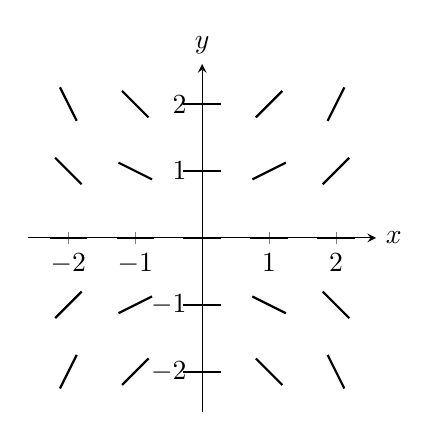
\begin{tikzpicture}
\begin{axis}[width=6cm,height=6cm,axis lines=middle,xmin=-2.6,xmax=2.6,ymin=-2.6,ymax=2.6,xtick={-2,-1,1,2},ytick={-2,-1,1,2},xlabel={$x$},ylabel={$y$},
 every axis x label/.style={at={(ticklabel* cs:1)},anchor=west},every axis y label/.style={at={(ticklabel* cs:1)},anchor=south}]
\foreach \i in {-2,...,2}{\foreach \j in {-2,...,2}{
  \pgfmathsetmacro{\m}{\i*\j/2}
  \pgfmathsetmacro{\dx}{0.28/sqrt(1+\m*\m)}
  \edef\temp{\noexpand\addplot[thick,domain=\i-\dx:\i+\dx,samples=2]{\j+\m*(x-\i)};}\temp
}}
\end{axis}
\end{tikzpicture}
\end{center}
The field for $\frac{dy}{dx}=\frac{xy}{2}$: horizontal segments along both axes, positive slopes in quadrants I and III, negative in II and IV. Solutions: $y=Ce^{x^2/4}$.
\end{example}

\section{Euler's method (7.5)}

\begin{rulebox}{R7.4}{Euler's method (BC)}
Start at $(x_0,y_0)$ with step $\Delta x$. Repeat: slope $m=\frac{dy}{dx}$ at the current point; $y_{\text{new}}=y+m\,\Delta x$; $x_{\text{new}}=x+\Delta x$. Show each step in a table. Euler's estimate follows tangent lines, so it underestimates when solution curves are concave up and overestimates when they are concave down.
\end{rulebox}

\begin{example}{two steps}
$\frac{dy}{dx}=x+y$, $y(0)=1$, $\Delta x=0.5$. Step 1: $m=0+1=1$, $y(0.5)\approx1+0.5=1.5$. Step 2: $m=0.5+1.5=2$, $y(1)\approx1.5+1=2.5$. (Exact: $2e-2\approx3.44$; the curve is concave up, so Euler underestimates.) \answer{$y(1)\approx2.5$.}
\end{example}

\section{Separation of variables (7.6--7.7)}

\begin{rulebox}{R7.5}{Separation of variables}
If $\frac{dy}{dx}=g(x)h(y)$, write $\frac{dy}{h(y)}=g(x)\,dx$ and integrate both sides; one constant $C$ is enough. Never split $\frac{dy}{dx}=x+y$: it is not separable.
\end{rulebox}

\begin{rulebox}{R7.6}{Particular solutions}
Use the initial condition to find $C$ \emph{right after integrating}, then solve for $y$. With $\ln|y|$, decide the sign from the initial condition. State the domain if asked: the largest interval containing $x_0$ on which the solution is defined.
\end{rulebox}

\begin{example}{separable equation}
$\frac{dy}{dx}=\frac{x}{y^2}$, $y(0)=2$. $\int y^2\,dy=\int x\,dx$: $\frac{y^3}{3}=\frac{x^2}{2}+C$; at $(0,2)$, $C=\frac83$. So $y^3=\frac{3x^2}{2}+8$. \answer{$y=\left(\frac32x^2+8\right)^{1/3}$.}
\end{example}

\begin{frqtip}
The separation question is usually worth 5 points: 1 for separating, 1 for each antiderivative, 1 for using the initial condition, 1 for solving for $y$. A response that does not separate correctly earns 0 of the 5. Keep the $+C$ and substitute the initial condition before solving for $y$.
\end{frqtip}

\section{Exponential and logistic models (7.8--7.9)}

\begin{rulebox}{R7.7}{Exponential growth and decay}
$\frac{dy}{dt}=ky$ has solutions $y=y_0e^{kt}$. $k>0$: growth, doubling time $\frac{\ln2}{k}$; $k<0$: decay, half-life $\frac{\ln2}{|k|}$. Newton's law of cooling $\frac{dT}{dt}=k(T-A)$ gives $T=A+(T_0-A)e^{kt}$.
\end{rulebox}

\begin{rulebox}{R7.8}{Logistic growth (BC)}
$\frac{dP}{dt}=kP\left(1-\frac PL\right)$ with $k>0$, $L>0$. The carrying capacity is $L$: if $0<P(0)<L$, $P$ increases toward $L$, and $\lim_{t\to\infty}P(t)=L$ (also if $P(0)>L$, decreasing toward $L$). $P$ grows fastest when $P=\frac L2$ (the vertex of $\frac{dP}{dt}$ as a function of $P$); the graph of $P$ has its inflection point there. Solution: $P=\frac{L}{1+Ae^{-kt}}$.
\end{rulebox}

\begin{example}{reading a logistic equation}
$\frac{dP}{dt}=0.4P-0.002P^2=0.4P\left(1-\frac{P}{200}\right)$. Carrying capacity 200; fastest growth when $P=100$; if $P(0)=50$, then $\lim_{t\to\infty}P=200$.
\end{example}

\section{Common errors}
\begin{itemize}
\item Writing $\frac{dy}{dt}=ky$ when the statement says proportional to something else (R7.1).
\item Using the slope at the new point instead of the current point in Euler's method (R7.4).
\item Adding $+C$ after solving for $y$ (``$y=e^{x^2}+C$'' instead of $y=Ce^{x^2}$) (R7.6).
\item Separating a non-separable equation (R7.5).
\item Giving $\frac L2$ as the limit instead of $L$ (R7.8).
\end{itemize}

\end{document}
